%ju 31-Dez-22 04-Generator.tex
\textbf{Drehstromgenerator / Lichtmaschine / Generator}

Quelle: Fabian Lindenberg, Kfz-Technik einfach erklärt \footnote{\url{https://www.youtube.com/watch?v=O7ydsAZ6bes}}

\section{Komponenten}\label{komponenten}

\begin{enumerate}
\item
  \textbf{Regler} (Multifunktionsregler hat keine Erregendioden, bekommt
  Spg. von Kl.30)
\item
  \textbf{Schleifringe}
\item
  \textbf{Gleichrichterdioden} (Leistungsdioden)
\item
  \textbf{Klauenpolläufer} (mit Riemenscheibe $\to$ Antrieb Motor und
  Schleifringe $\to$ Regler)
\item
  \textbf{Erregerwicklung} (Rotor, dreht sich, sitzt im Klauenpolläufer)
\item
  \textbf{Ständerwicklung} (mit Gehäuse, Stator, steht)
\item
  \textbf{Lüfter}
\end{enumerate}

\textbf{Diodenplatte:} 6x Gleichrichterdioden (3x Plusdioden, 3x
Minusdioden), 3x Erregerdioden

\textbf{Klauenpolläufer} 12 Pole (je 6 Nord- und Südpole) x 3
Statorspulen = 36 Halbwellen = 1x Umdrehung. Batterie und Kondensator
glättet die Gleichspannung.

\begin{figure}[!ht]% hier: !ht
\centering
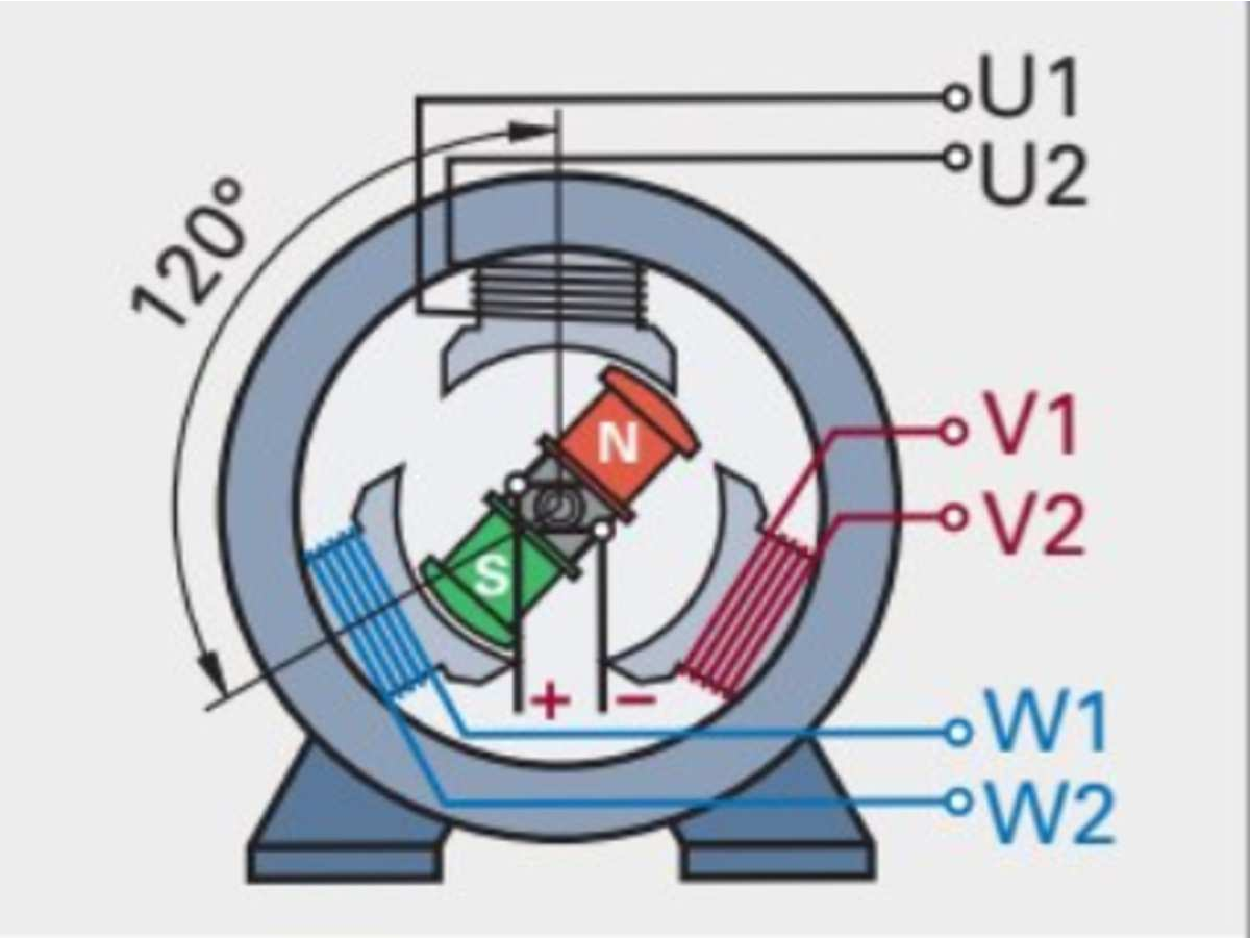
\includegraphics[width=0.4\textwidth]{images/Generator/Generator-11.pdf}
\caption{Generatoraufbau - Drei Ständerwicklungen U,V,W und ein Polrad}
%\label{fig:}%% anpassen
\end{figure}

\begin{figure}[!ht]% hier: !ht
\centering
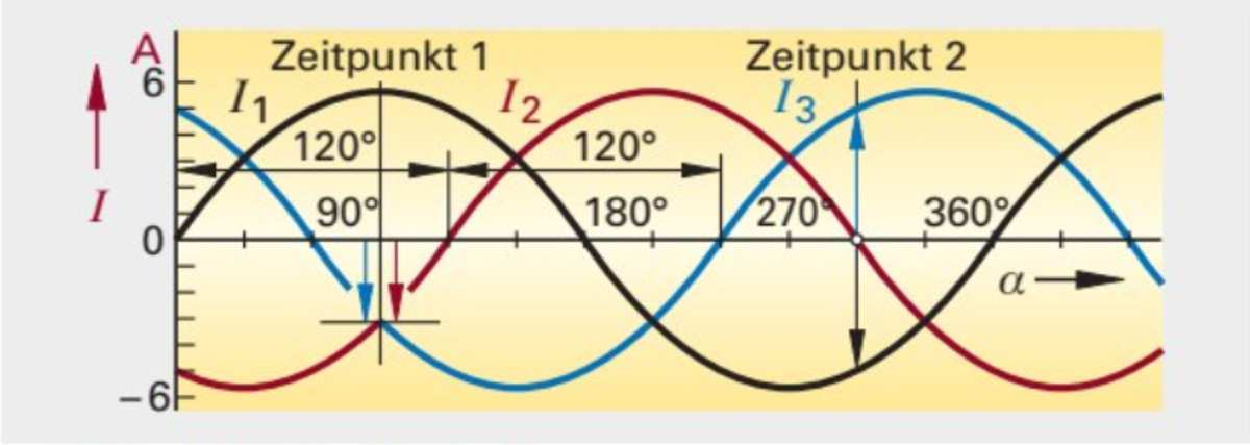
\includegraphics[width=0.4\textwidth]{images/Generator/Generator-8.pdf}
\caption{3 Wechselspannungen mit 120° Phasenverschiebung}
%\label{fig:}%% anpassen
\end{figure}

\section{Multifunktionsregler}\label{multifunktionsregler}

\begin{figure}[!ht]% hier: !ht
\centering
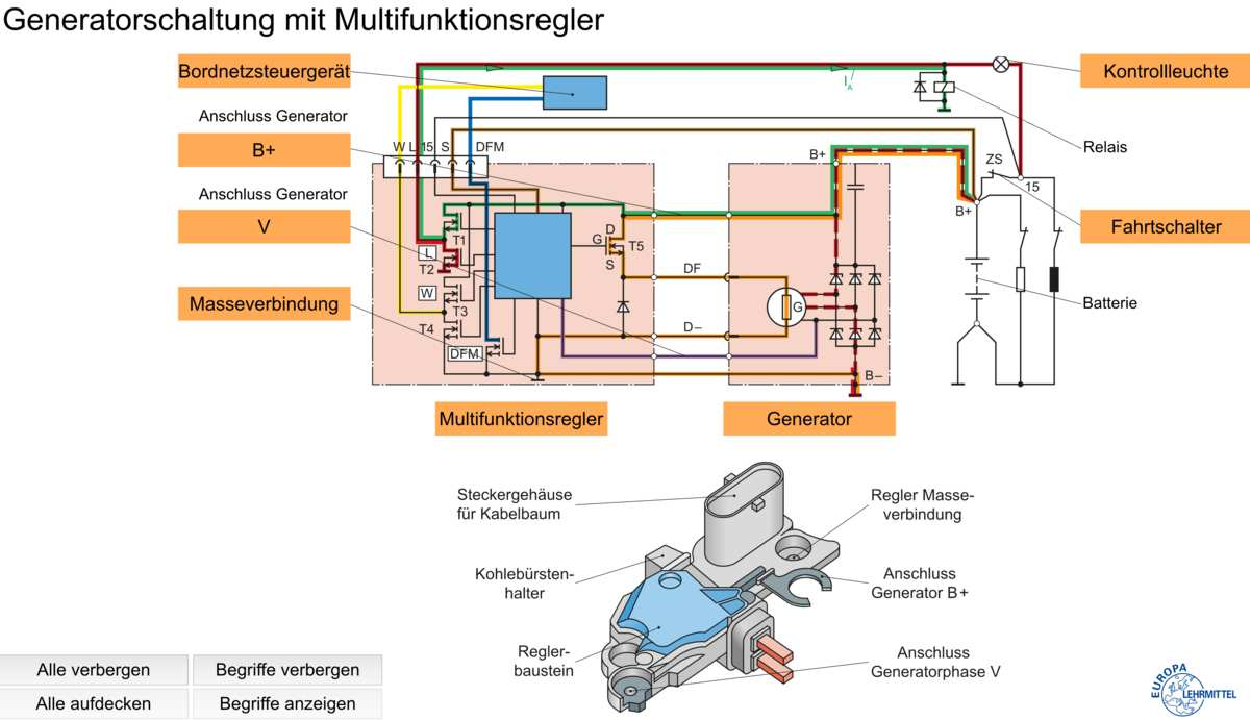
\includegraphics[width=0.85\textwidth]{images/Generator/Generator-1.pdf}
\caption{Schaltung Generator mit Multifunktionsregler, Quelle:
Europa-Verlag}
%\label{fig:}%% anpassen
\end{figure}

\textbf{Merkmale}

\begin{enumerate}
\item
  Unterstützung Motormanagement
\item
  Batterieüberwachung
\item
  Auslastungsüberwachung
\item
  Temperaturabhängige Ladespannung
\item
  Schutz gegen Überlastung / Kurzschluss
\item
  Interne Fehlerdiagnose $\to$ SG
\item
  Vorerregerstrom Steuern (Dreht sich der Generator)
\item
  Low-Response (Start \& Fahrt: Belastung des Generators wird verzögert
  zugeschaltet, Kraftstoff sparen)
\end{enumerate}

\newpage

\section{Generator prüfen}\label{generator-pruefen}

\textbf{Ladekontrolle an}

\begin{itemize}
\item
  Zündung an, Motor steht
\item
  Erregungsunterbrechung
\item
  Überspannung
\item
  Keilriemen gerissen
\item
  Leitungsunterbrechung
\item
  Defekte Masseverbindung
\end{itemize}

\textbf{Generator Anschluss}

\begin{enumerate}
\item
  \textbf{W} Drehzahl
\item
  \textbf{B-} Masse
\item
  \textbf{D+} Ladekontrolle, Erregerwicklung
\item
  \textbf{B+} Batterie
\item
  \textbf{DF} Regler, Erregerwicklung
\end{enumerate}

\textbf{Generator mit Multifunktionsregler Anschluss}

\begin{enumerate}
\item
  \textbf{L} Ladekontrollleuchte
\item
  \textbf{S} Sense, Batterie überwachen
\item
  \textbf{W} Drehzahlsignal zur Regelung des Vorerregerstroms
\item
  \textbf{V} Phasenspannung überwachen (Fehlerdiagnose, Beispiel: def.
  Keilriemen erkennen)
\item
  \textbf{DFM} PWM-Signal des Erregerstroms zur Auslastung des
  Generators
\end{enumerate}

\textbf{Erregerspannung und Generatorspannung / Ladespannung messen}

\begin{itemize}
\item
  Unter Belastung (Verbraucher EIN)
\item
  Motordrehzahl (ca. 1800 - 2200 1/min)
\item
  \textbf{Erregerspannung}

  \begin{itemize}
  \item
    Messpunkt: (D+ und D-/B-/Masse)
  \end{itemize}
\item
  \textbf{Generatorspannung / Ladespannung}

  \begin{itemize}
  \item
    Messpunkt: (B+ und D-/B-/Masse)
  \end{itemize}
\end{itemize}

\textbf{Fehler}

\begin{enumerate}
\item
  Oberwelle normal
\item
  Minusseitig eine Sperrdiode defekt $\to$ Eine Welle wäre weg,
  Leistung von der Spule fehlt
\item
  Erregerdiode defekt $\to$ Ladespannung geht runter
\end{enumerate}

\begin{figure}[!ht]% hier: !ht
\centering
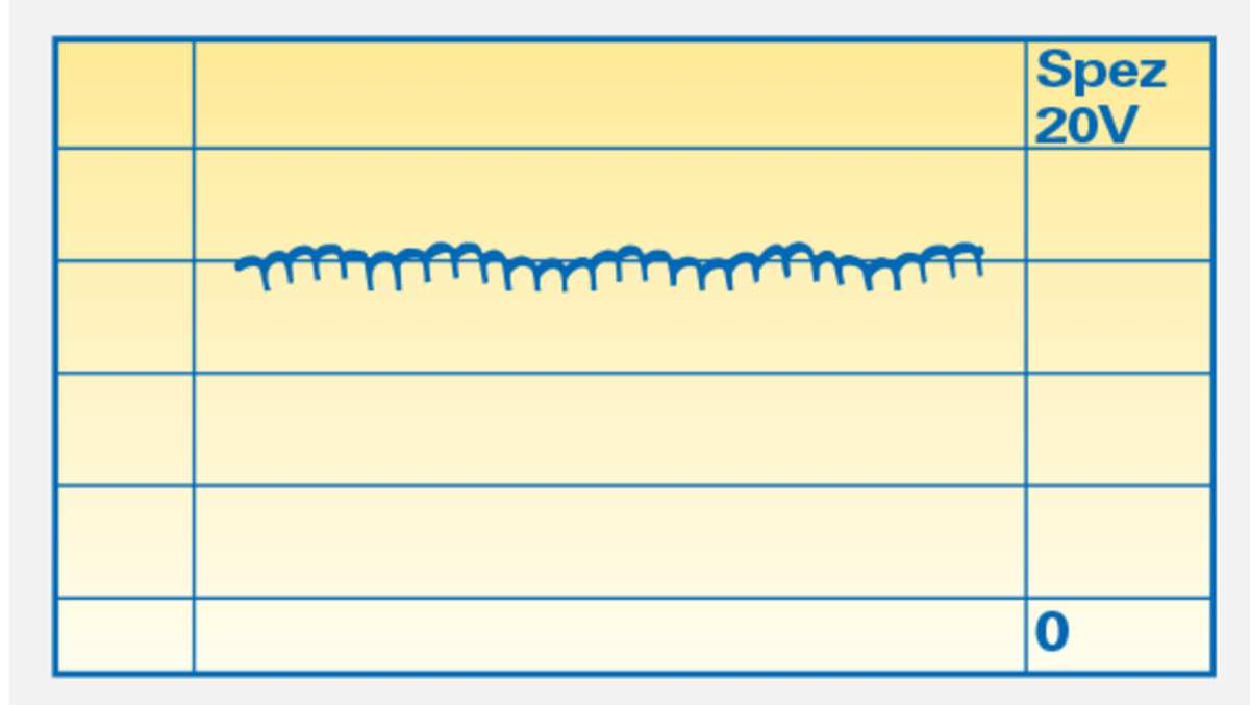
\includegraphics[width=0.4\textwidth]{images/Generator/Generator-2.pdf}
\caption{Generator Gutbild, Quelle: Europa-Verlag}
%\label{fig:}%% anpassen
\end{figure}

\begin{figure}[!ht]% hier: !ht
\centering
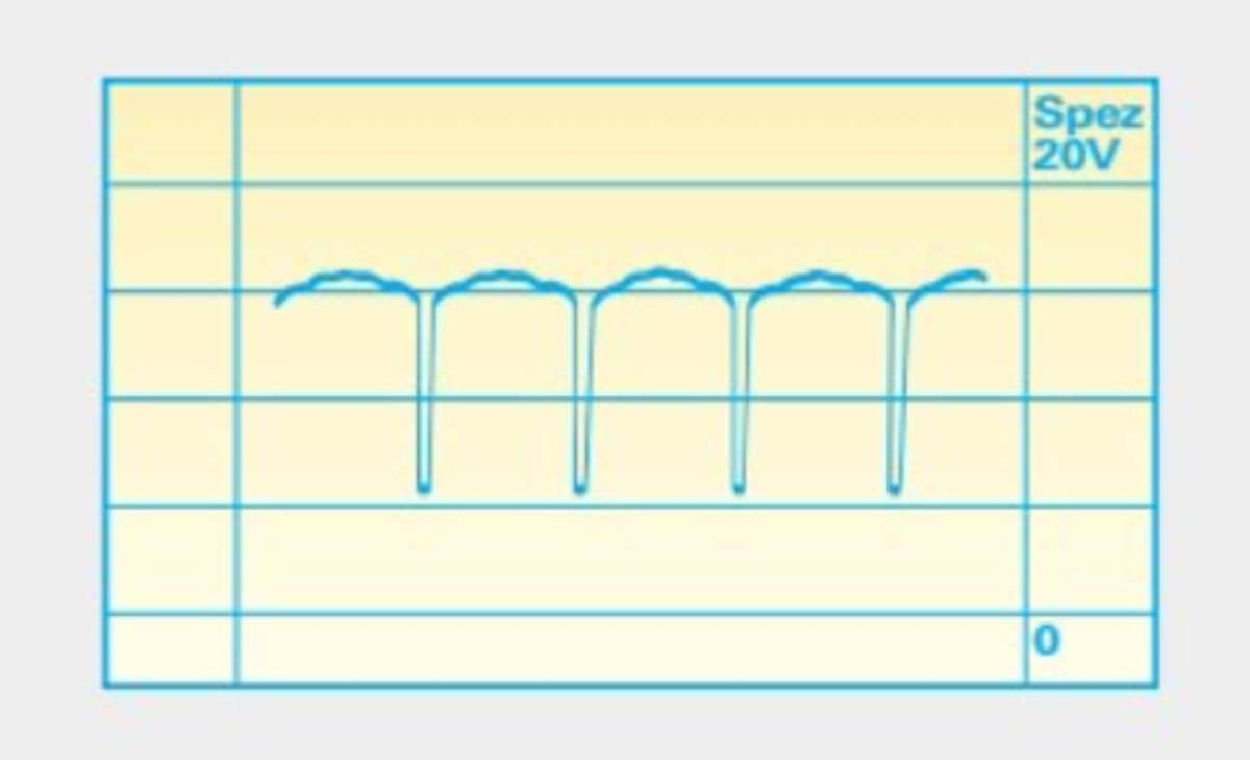
\includegraphics[width=0.4\textwidth]{images/Generator/Generator-5.pdf}
\caption{Generator Fehler - Unterbrechung einer Minusdiode, Quelle:
Europa-Verlag}
%\label{fig:}%% anpassen
\end{figure}

\newpage

\section{Energieumwandlung}\label{energieumwandlung}

kinetische Energie + elektrische Energie (Drehmoment) $\to$
\textbf{Generator} $\to$ elektrische Energie

\textbf{Induktion} mit ein Magnetfeld Elektronen bewegen.

Magnet (Nordpol/Südpol, anziehen / abstoßen)

Rechte-Handregel: Magnetfeld bestimmen

\begin{enumerate}
\item
  Stromdurchflossener Leiter $\to$ erzeugt Magnetfeld
\item
  Stromdurchflosse Spule $\to$ erzeugt großes Magnetfeld
\item
  Rotor (Erregerwicklung, Fremderregt) und Stator (mit 3x Spulen, U / V
  / W) $\to$ erzeugt drehbares Magnetfeld
\end{enumerate}

\textbf{indizierte Spannung} ist abhängig

\begin{enumerate}
\item
  Anzahl Wicklungen von Statorspulen
\item
  Drehzahl Generator
\item
  Stärke des Magnetfeldes
\item
  Fläche
\end{enumerate}

\begin{figure}[!ht]% hier: !ht
\centering
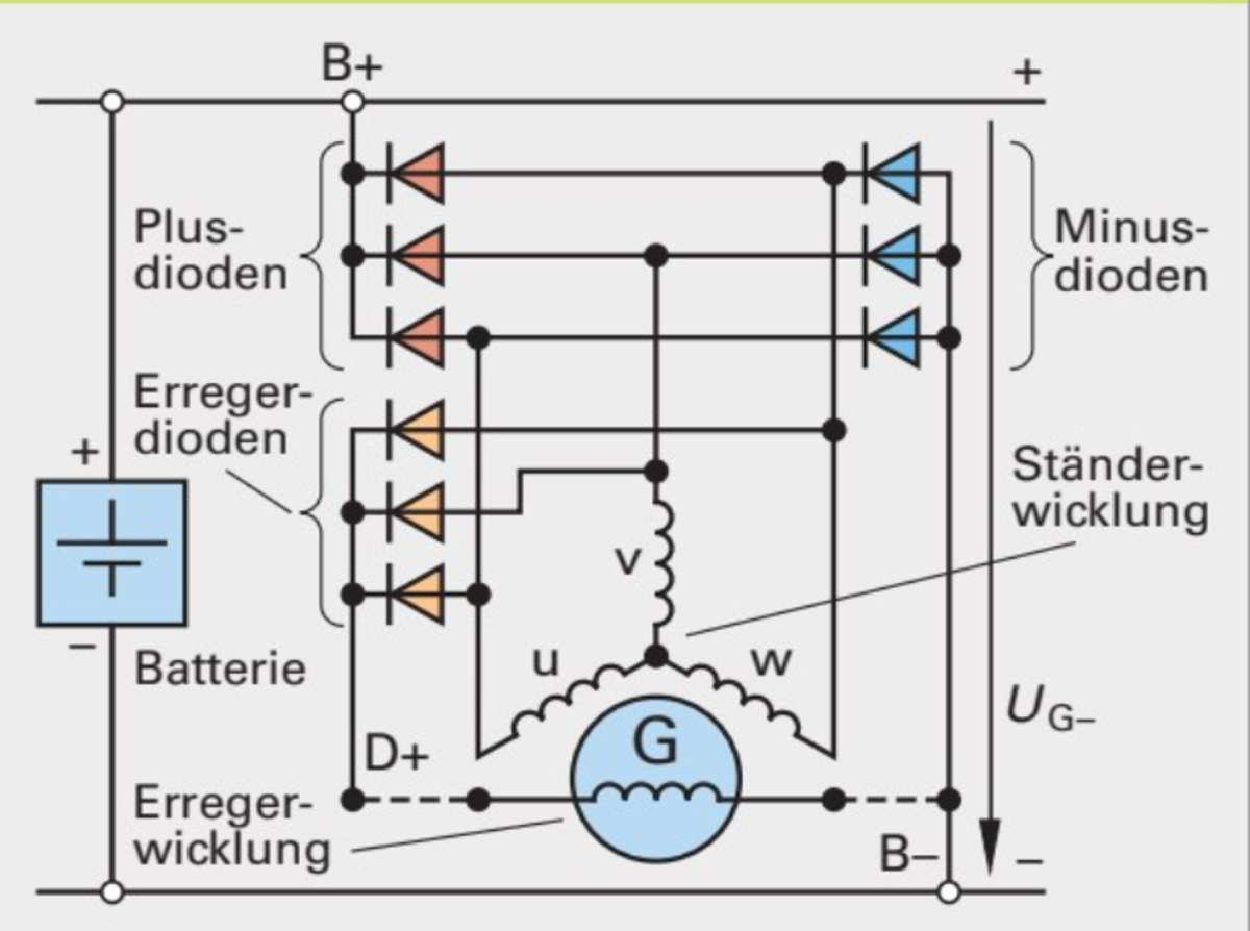
\includegraphics[width=0.3\textwidth]{images/Generator/Generator-6.pdf}
\caption{Drehstrom - Brückenschaltung}
%\label{fig:}%% anpassen
\end{figure}

\begin{figure}[!ht]% hier: !ht
\centering
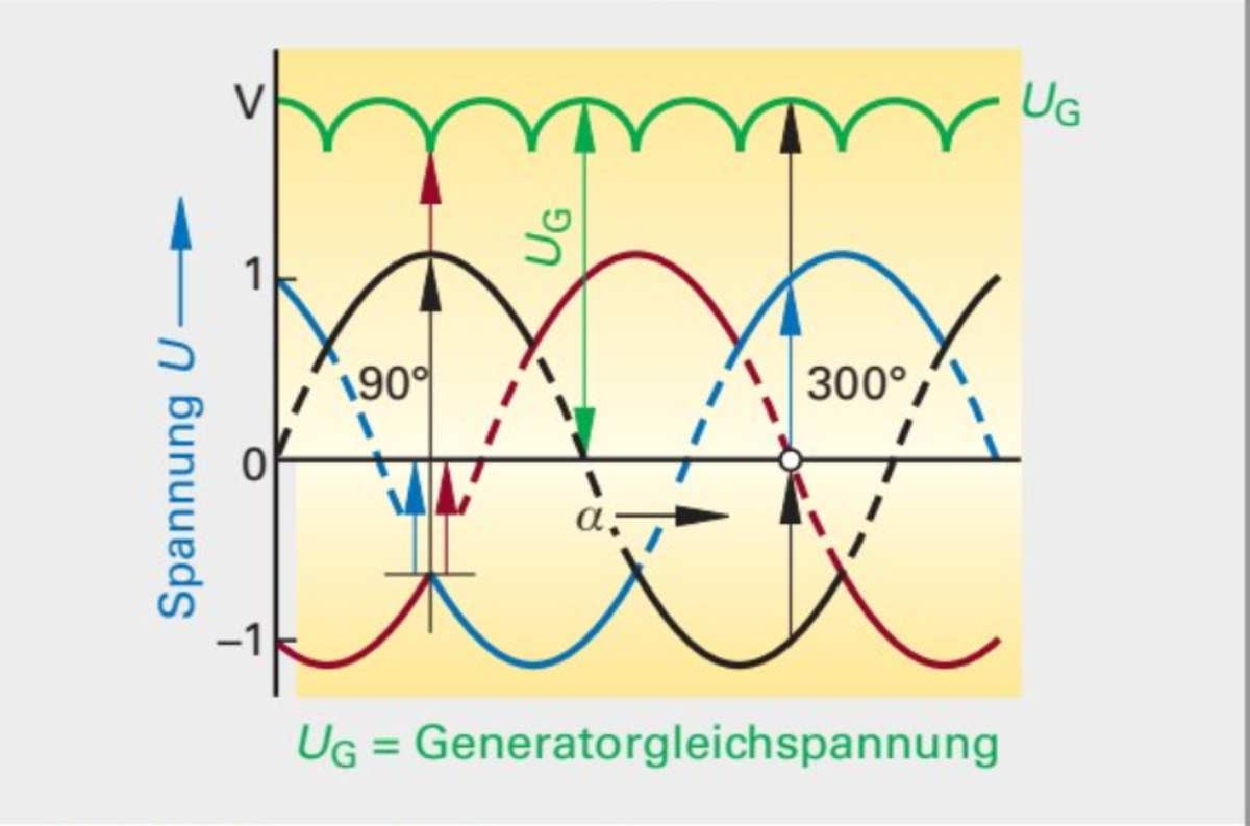
\includegraphics[width=0.3\textwidth]{images/Generator/Generator-7.pdf}
\caption{Gleichrichtung der Generatorspannung}
%\label{fig:}%% anpassen
\end{figure}

\newpage

\section{Energiefluss}\label{energiefluss}

\begin{figure}[!ht]% hier: !ht
\centering
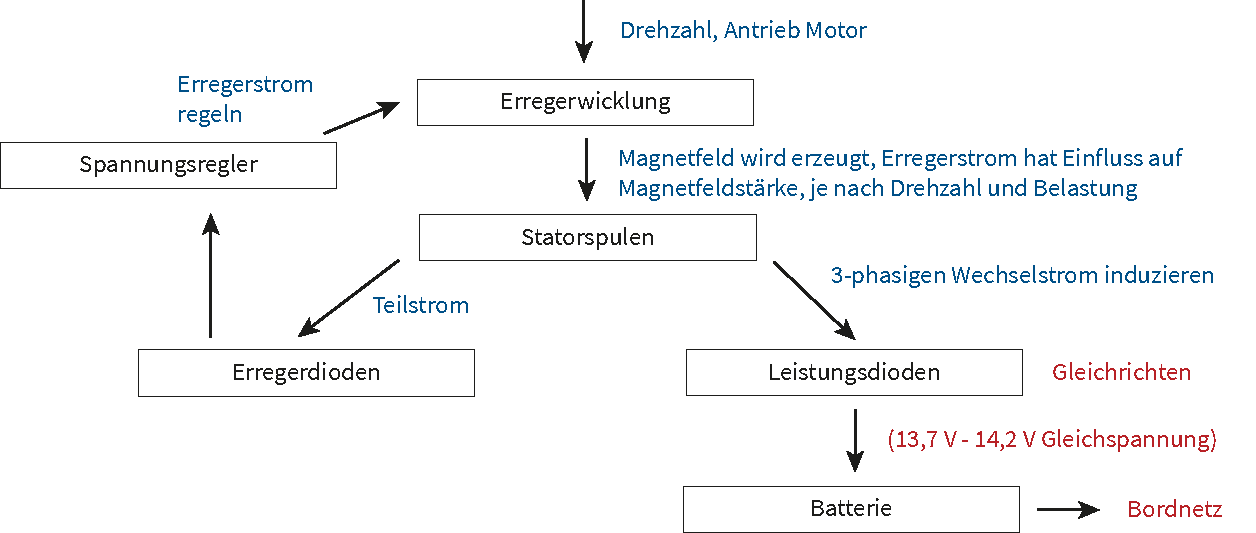
\includegraphics[width=0.8\textwidth]{images/Generator/Generator-Energiefluss.pdf}
\caption{Energiefluss}
%\label{fig:}%% anpassen
\end{figure}

\textbf{Erregerwicklung} sitzt im Klauenpolläufer, erzeugt Magnetfeld
welches auf die Statorspulen wirkt

\textbf{Statorspulen} Sternschaltung, Durch das Magnetfeld der
Erregerwicklung wird eine Spannung induziert. 3x Spulen um 120° versetzt
$\to$ 3-phasige Wechselspannung

\textbf{Leistungsdioden} Richten die 3-phasige Wechselspannung in eine
Gleichspannung um.

\textbf{Erregerdioden} Spannungsversorgung des Spannungsreglers.

\textbf{Spannungsregler} regelt den Erregerstrom und variiert damit die
Stärke des Magnetfeldes. \textbf{Ladespannung ist Konst.} bei allen
Motordrehzahlen (Leerlauf - Vollast) u. Belastungen (Verbraucher).
\textbf{Wie?} Je stärker das Magnetfeld, desto größer ist die Spannung
die in den Statorspulen induziert wird.

\newpage

\section{Schaltung}\label{schaltung}

\begin{figure}[!ht]% hier: !ht
\centering
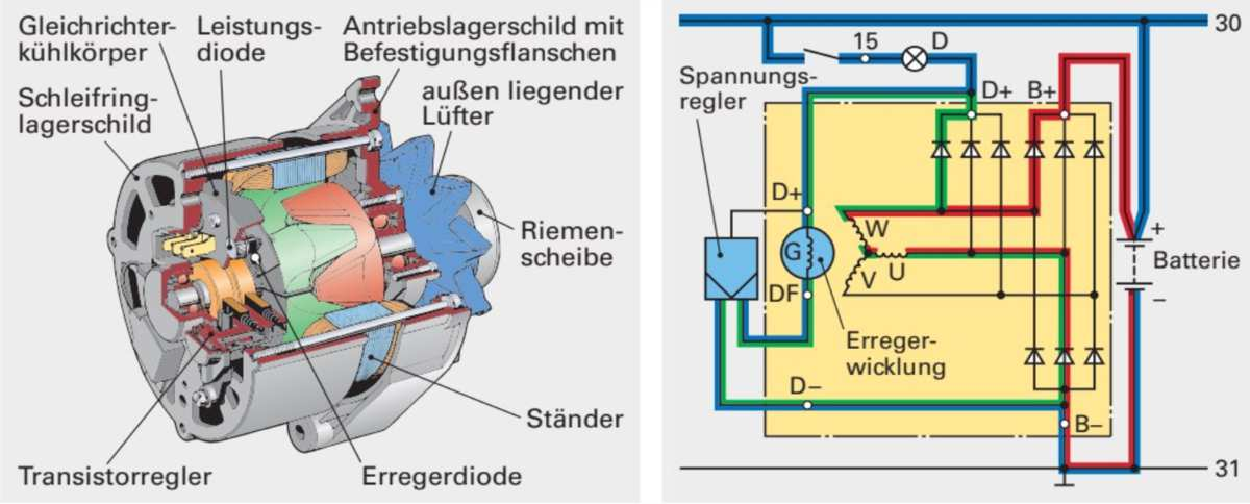
\includegraphics[width=0.85\textwidth]{images/Generator/Generator-9.pdf}
\caption{Schaltung Generator mit Transistorregler, Quelle:
Europa-Verlag}
%\label{fig:}%% anpassen
\end{figure}

Zündung an, Motor steht

\textbf{Vorerregerstromkreis (blau)} B+ $\to$ Fahrtschalter $\to$
Ladekontrolllampe $\to$ D+ $\to$ Erregerwicklung $\to$ Regler DF
$\to$ Masse $\to$ B-

Zündung an, Motor läuft

\textbf{Erregerstromkreis (grün)} Ständerwicklung $\to$ Erregerdioden
$\to$ D+ $\to$ Erregerwicklung $\to$ Regler DF $\to$ Regler D-
$\to$ Minusdioden $\to$ Ständerwicklung

\textbf{Ladestromkreis (rot)} Ständerwicklung $\to$ Plusdioden $\to$
B+ $\to$ Verbraucher $\to$ Masse $\to$ Minusdioden $\to$
Ständerwicklung

\newpage

\begin{figure}[!ht]% hier: !ht
\centering
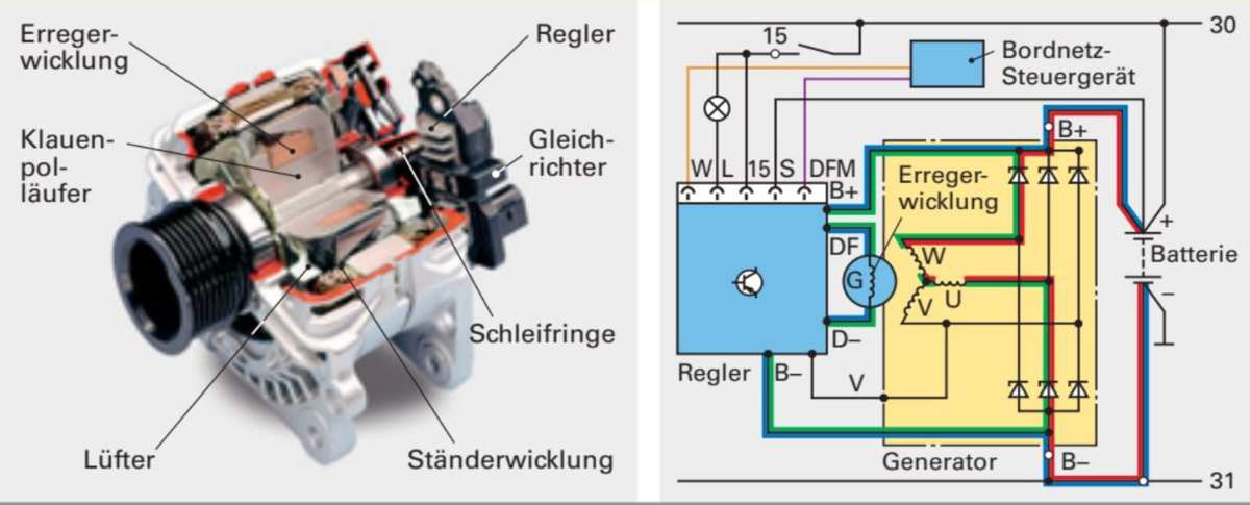
\includegraphics[width=0.85\textwidth]{images/Generator/Generator-10.pdf}
\caption{Schaltung Generator mit Multifunktionsregler, Quelle:
Europa-Verlag}
%\label{fig:}%% anpassen
\end{figure}

\textbf{Vorerregerstromkreis (blau)} B+ $\to$ Erregerwicklung $\to$
Regler DF $\to$ Reglerendstufe $\to$ B-

Zündung an, Motor läuft

\textbf{Erregerstromkreis (grün)} Ständerwicklung $\to$ Plusdioden
$\to$ Regler B+ $\to$ Regler DF $\to$ Erregerwicklung $\to$
Regler D- $\to$ Regler B- $\to$ Minusdioden $\to$ Ständerwicklung

\textbf{Ladestromkreis (rot)} Ständerwicklung $\to$ Plusdioden $\to$
B+ $\to$ Verbraucher $\to$ Masse $\to$ Minusdioden $\to$
Ständerwicklung
